\documentclass[a4paper]{jpconf}
\usepackage{graphicx}

% Packages physics of fluids 
\usepackage{tabularx}
\usepackage{multirow}

\usepackage{booktabs,caption,fixltx2e}
\usepackage[flushleft]{threeparttable}


\usepackage{arydshln}

% Packages philtrans
\usepackage{mathrsfs}
\usepackage{amsmath}
\usepackage{amsfonts}
\usepackage{epstopdf}
\usepackage{etoolbox}
\usepackage{tikz}
\usepackage[outline]{contour}
\newcommand{\addref}{{\color{blue} REF}}
\newcommand{\ufilt}{\tilde{\boldsymbol{u}}}
\newcommand{\commwim}[1]{{\color{red} #1}}
\newcommand{\dx}{\text{d}\boldsymbol{x}}
\newcommand{\dt}{\text{d}t}
\newcommand{\ddd}{\text{d}}
\newcommand{\ddt}[1]{\frac{\ddd #1}{\ddd t}}
\newcommand{\blds}[1]{\boldsymbol{#1}}
\newcommand{\dd}[2]{\frac{\ddd #1}{\ddd #2}}
\newcommand{\ctihat}{\widehat{C}_{T,i}'}
\newcommand{\cthat}{\widehat{C}_T'}
\newcommand{\ctmax}{C_{T,\text{max}}'}

\newcommand{\legend}{(\emph{Legend}: R: {\bf \color{black}-----}, C3t0: {\bf \color{red}-----}, C3t5: {\bf\color{Dandelion}-----}, C3t30: {\bf\color{Cyan}-----}, C2t0: {\bf\color{red}- - -}, C2t5: {\bf\color{Dandelion}- - -}, C2t30: {\bf\color{Cyan}- - -})}
\newcommand{\legendtauref}{(\emph{Legend}: R: {\bf \color{black}-----}, $\tau = 0$ s: {\bf \color{red}-----}, $\tau = 5$ s: {\bf\color{Dandelion}-----}, $\tau = 30$ s: {\bf\color{Cyan}-----})}

\newcommand{\legendnoref}{C3t0: {\bf \color{red}-----}, C3t5: {\bf\color{Dandelion}-----}, C3t30: {\bf\color{Cyan}-----}, C2t0: {\bf\color{red}- - -}, C2t5: {\bf\color{Dandelion}- - -}, C2t30: {\bf\color{Cyan}- - -}}

\newcommand{\legendtau}{(\emph{Legend}: $\tau = 0$ s: \contour{red}{\color{red}-----}, $\tau = 5$ s: \contour{Dandelion}{\color{Dandelion}-----}, $\tau = 30$ s: \contour{Cyan}{\color{Cyan}-----})}
%\newcommand{\legendtauref}{(\emph{Legend}: R: \contour{black}{\color{black}-----}, $\tau = 0$ s: \contour{red}{\color{red}-----}, $\tau = 5$ s: \contour{Dandelion}{\color{Dandelion}-----}, $\tau = 30$ s: \contour{Cyan}{\color{Cyan}-----})}

\newrobustcmd*{\mycircle}[1]{\tikz{\filldraw[draw=#1,fill=#1] (0,0) 
		circle [radius=0.08cm];}}
\newrobustcmd*{\mycircleopen}[1]{\tikz{\filldraw[draw=#1,fill=white] (0,0) circle [radius=0.08cm];}}

% Yawing paper
% Additional packages to be loaded
%---------------------------------------------------------------------------------
\usepackage{mathtools}
\usepackage{mathrsfs}
\usepackage{amsmath}
\usepackage[short]{optidef}
\usepackage{printlen}
\usepackage{tikz}
\usepackage{xcolor}

\definecolor{C1}{RGB}{31,119,180}
\definecolor{C2}{RGB}{255,127,14}
\definecolor{C3}{RGB}{44,160,44}
\definecolor{C4}{RGB}{214,39,40}

% Some  auxiliary commands for ease of mathematics notations
%---------------------------------------------------------------------------------
% Derivatives and differentials
\newcommand{\ds}{~\text{d}\boldsymbol{s}}
\newcommand{\dzeta}{~\text{d}\boldsymbol{\zeta}}
\newcommand{\pder}[2]{\frac{\partial #1}{\partial #2}}
\newcommand{\bolds}[1]{\boldsymbol{#1}}
% Integrals
\newcommand{\stint}{\int_{0}^{T} \int_{\Omega}}
\newcommand{\sint}{\int_{\Omega}}
\newcommand{\Tint}{\int_{0}^{T}}
\newcommand{\tint}{\int_{0}^{t}}
% Filtered variables
\newcommand{\utilde}{\widetilde{\bolds{u}}}
\newcommand{\ptilde}{\widetilde{p}}
\newcommand{\ctnhat}[1]{\widehat{C}_{T,#1}'}
% Other symbols
\newcommand{\cti}{C_{T,i}'}
\newcommand{\ctn}[1]{C_{T,#1}'}
\newcommand{\R}{\mathscr{R}}
\newcommand{\J}{\mathscr{J}}
\newcommand{\Jtilde}{\tilde{\mathscr{J}}}
\newcommand{\Jgrad}{\nabla \Jtilde}
\newcommand{\Lagr}{\mathscr{L}}
\newcommand{\eperp}{\bolds{e}_\perp}
\newcommand{\eperpi}{\bolds{e}_{\perp,i}}
\newcommand{\etransi}{\bolds{e}_{\parallel,i}}
\newcommand{\ex}{\bolds{e}_x}
\newcommand{\ey}{\bolds{e}_y}
\newcommand{\ez}{\bolds{e}_z}
\newcommand{\eperpn}[1]{\bolds{e}_{\perp,#1}}
\newcommand{\vi}{\frac{1}{A_i} \sint \R_i (\bolds{s})~\utilde \cdot \eperpi \ds}
% Operators
\newcommand{\innerproduct}[2]{\bigg( #1, #2 \bigg)}
\newcommand{\innerproductsmall}[2]{\big( #1, #2 \big)}
\newcommand{\sumturbines}{\sum_{i=1}^{N_t}}
\newcommand{\diracdelta}{{\delta}}
% Colors
\newcommand{\red}[1]{{\color{red} #1}}
\newcommand{\purp}[1]{{\color{purple} #1}}
\newcommand{\reftodo}[1]{\red{AddREF}: #1}
\newcommand{\todo}[1]{\purp{TODO: #1}}
\newcommand{\fixeqref}{\purp{FixEqRef}}
%---------------------------------------------------------------------------------

%---------------------------------------------------------------------------------
\usepackage{mathtools}
\usepackage{mathrsfs}
\usepackage{amsmath}
\usepackage[short]{optidef}
\usepackage{printlen}
\usepackage{tikz}
\usepackage{xcolor}

\definecolor{C1}{RGB}{31,119,180}
\definecolor{C2}{RGB}{255,127,14}
\definecolor{C3}{RGB}{44,160,44}
\definecolor{C4}{RGB}{214,39,40}
\DeclareMathOperator*{\argmin}{arg\,min}

\newcommand{\sqdiamond}[1][fill=gray]{\tikz [x=1.2ex,y=1.85ex,line width=.1ex,line join=round, yshift=-0.285ex] \draw  [#1]  (0,.5) -- (.5,1) -- (1,.5) -- (.5,0) -- (0,.5) -- cycle;}%
\newcommand{\miDiamond}[1][fill=gray]{\mathop{\raisebox{-0.275ex}{$\sqdiamond[#1]$}}}



\begin{document}
\title{Optimal dynamic induction and yaw control of wind farms: effects of turbine spacing and layout}

\author{Wim Munters and Johan Meyers}

\address{Department of Mechanical Engineering, KU Leuven, Celestijnenlaan 300A, B3001 Leuven, Belgium}

\ead{wim.munters@kuleuven.be, johan.meyers@kuleuven.be}

\begin{abstract}
Turbine wake interactions in wind farms result in decreased power extraction in downstream rows. The current work investigates dynamic induction and yaw control of wind farms for increased total power extraction. Six different wind farm layouts are considered, and the relative benefits of induction control, yaw control, and combined induction--yaw control are compared. Preliminary results show that, through coordinated induction control, turbine density can be increased significantly with the same wind-farm efficiency as an uncoordinated farm.
\end{abstract}

\section{Introduction}
Turbine wake interactions in wind farms result in decreased power extraction in downstream rows. The promise of increasing total power extraction through coordinated wind-farm control has incited a multitude of studies into axial induction control and yaw control of wind turbines. In earlier work \cite{goit, munters}, a dynamic induction control approach was introduced based on large-eddy simulations and optimization. Recently, this approach was expanded to also include yaw \cite{phd}. A control study of a $4 \times 4$ wind farm with 6 rotor diameters spacing illustrated that yaw control tends to be more favorable than induction control for small sets of aligned wind turbines, and that combining yaw and induction control potentially further increases power gains. 

In the current work, we aim to quantify and compare the potential power gains for induction control, yaw control and combined induction--yaw control in large wind farms with both aligned and staggered layouts. Especially in the latter, the abovementioned advantage of yaw control over induction control is expected to be diminished, since yaw could lead to detrimental interactions between different columns of wind turbines by transversally deflected turbine wakes. Furthermore, control studies are also performed for wind farms with an increased turbine density, where the effect of turbine wake interactions on wind-farm power is further increased.  

 \section{Methodology}

We apply a receding-horizon model-predictive control approach with a  large-eddy simulation flow model, in which wind-farm operation is optimized over a total time of 30 minutes, consisting of 15 sequential windows with a prediction horizon $T = 240$~s and a control application time $T_A = T/2 = 120$~s (see Ref. \cite{munters}). To this end, we consider the following PDE-constrained optimization problem:

\begin{alignat}{4}
& \underset{\bolds{\varphi}, \bolds{q}}{\text{min}}  & \qquad  \J(\bolds{\varphi}, \bolds{q}) &= - \Tint \sum_{i=1}^{N_t} \frac{1}{2} \ctihat~V_i^3 A_i \dt  & \label{eq:costfunction}\\
& \text{s.t.}                      			&         \frac{\partial \utilde}{\partial t} + \big(\utilde \cdot \nabla \big)~ \utilde &= - \nabla (\ptilde + \ptilde_\infty) / \rho - \nabla \cdot \boldsymbol{\tau}_{sgs} + \sum_{i=1}^{N_t} \bolds{f}_i \qquad  & \text{in } \Omega \times (0,T], \label{eq:NSmomentum_constraint} \\
&                                                   &        \nabla \cdot \utilde&=0 									        & \text{in } \Omega \times (0,T], \label{eq:NScontinuity_constraint}\\
&                                                   &        \tau \ddt{\ctihat}&=\cti - \ctihat 								& i=1\dots N_t~\text{in } (0,T],  \label{eq:ctihat_constraint}\\
&                                                   &        \ddt{\theta_i}&=\omega_i											& i=1\dots N_t~\text{in } (0,T],  \label{eq:omega_constraint}\\
&                                                   &        C_{T,\text{min}}' \leq~ &\cti \leq C_{T,\text{max}}'				& i=1\dots N_t~\text{in } (0,T],  \label{eq:boxct_constraint}\\
&                                                   &        -\omega_{\text{max}} \leq~ &\omega_i \leq \omega_{\text{max}}.   	& i=1\dots N_t~\text{in } (0,T],  \label{eq:boxomega_constraint}
\end{alignat}
with system states $\bolds{q}(\bolds{x},t) = [\ufilt(\bolds{x},t),\ \ptilde(\bolds{x},t),\ \ctnhat{1}(t), \dots, \ctnhat{N_t}(t), \theta_1(t), \dots, \theta_{N_t}(t)]$ and controls $\bolds{\varphi}(t)~=~[\ctn{1}(t), \dots, \ctn{N_t}(t), \omega_1(t), \dots, \omega_{N_t}(t)]$. State equations (\ref{eq:NSmomentum_constraint} -- \ref{eq:NScontinuity_constraint}) are the filtered Navier--Stokes equations modeling the turbulent wind-farm boundary layer. In these equations, $\ufilt$ and $\ptilde$ are the filtered velocity and pressure respectively. Further, $\nabla \ptilde_\infty$ is the driving background pressure gradient and $\bolds{\tau}_{\rm sgs}$ is the subgrid-scale stress tensor. The thrust force $\bolds{f}_i$ enacted on the flow by each turbine $i$ is modeled using an actuator disk approach as 
%\begin{equation}
$\bolds{f}_i = \frac{1}{2} \ctihat V_i^2 \R_i \eperpi$,
%\end{equation}
with $\ctihat$ the thrust coefficient, $\R_i$ the geometric footprint of the turbine on the LES grid, and $V_i = (1/A_i) \sint \R_i \utilde \cdot \eperpi \dx$ the disk-averaged velocity. The rotor-perpendicular vector $\eperpi = \bolds{e}_x \cos \theta_i + \bolds{e}_y \sin \theta_i$, with $\theta_i$ the turbine yaw angle. 
The thrust coefficient $\ctihat$ is obtained from its setpoint value $\cti$ through an exponential time filter with characteristic turbine response time $\tau = 5$ s (Eq. \ref{eq:ctihat_constraint}), and the turbine yaw angle is found through integration of the yaw rate $\omega_i$ (Eq. \ref{eq:omega_constraint}). Finally, controls are bound to technical box constraints in Eqs. (\ref{eq:boxct_constraint} - \ref{eq:boxomega_constraint}).
The optimization problem is solved in a reduced formulation using the L--BFGS--B algorithm, and the cost functional gradient is evaluated using the continuous adjoint method. 

\section{Case Setup \& Preliminary Results}

A total of six wind farms is investigated, comprised of three layouts with two different spacings. Figure \ref{fig:wf_layouts} illustrates the wind farms for the aligned (A), two-row staggered (St2), and three-row staggered (St3) cases. For each of these layouts, a wide (W) spacing and tight (T) spacing arrangement is considered, where the distance between adjacent turbine rows and columns is $S_W = 6D$ and $S_T = 3.6D$ respectively. This results in a turbine density of $3.03$~km$^{-2}$ for the wide spacing layouts, and $8.42$~km$^{-2}$ for the tight spacing layouts. For each farm, four control cases are considered: 
a greedy reference case R, with $(C_{T}'=2, \omega_{\rm max} = 0)$,
an inductive control case I $(0 \leq C_{T}' \leq 3, \omega_{\rm max} = 0)$,
a yaw control case Y $(C_{T}'=2, \omega_{\rm max} = 0.3)$,
and a combined inductive-yaw control case IY, with $(0 \leq C_{T}' \leq 3, \omega_{\rm max} = 0.3)$. 

%\begin{itemize}
%	\item a greedy reference case R, with $(C_{T, \rm min}', C_{T, \rm max}', \omega_{\rm max}) = (2, 2, 0)$,
%	\item an inductive control case I, with $(C_{T, \rm min}', C_{T, \rm max}', \omega_{\rm max}) = (0, 3, 0)$,
%	\item a yaw control case Y, with $(C_{T, \rm min}', C_{T, \rm max}', \omega_{\rm max}) = (2, 2, 0.3)$,
%	\item and a combined inductive-yaw control case IY, with $(C_{T, \rm min}', C_{T, \rm max}', \omega_{\rm max}) = (0, 3, 0.3)$. 
%\end{itemize}

\begin{figure}
	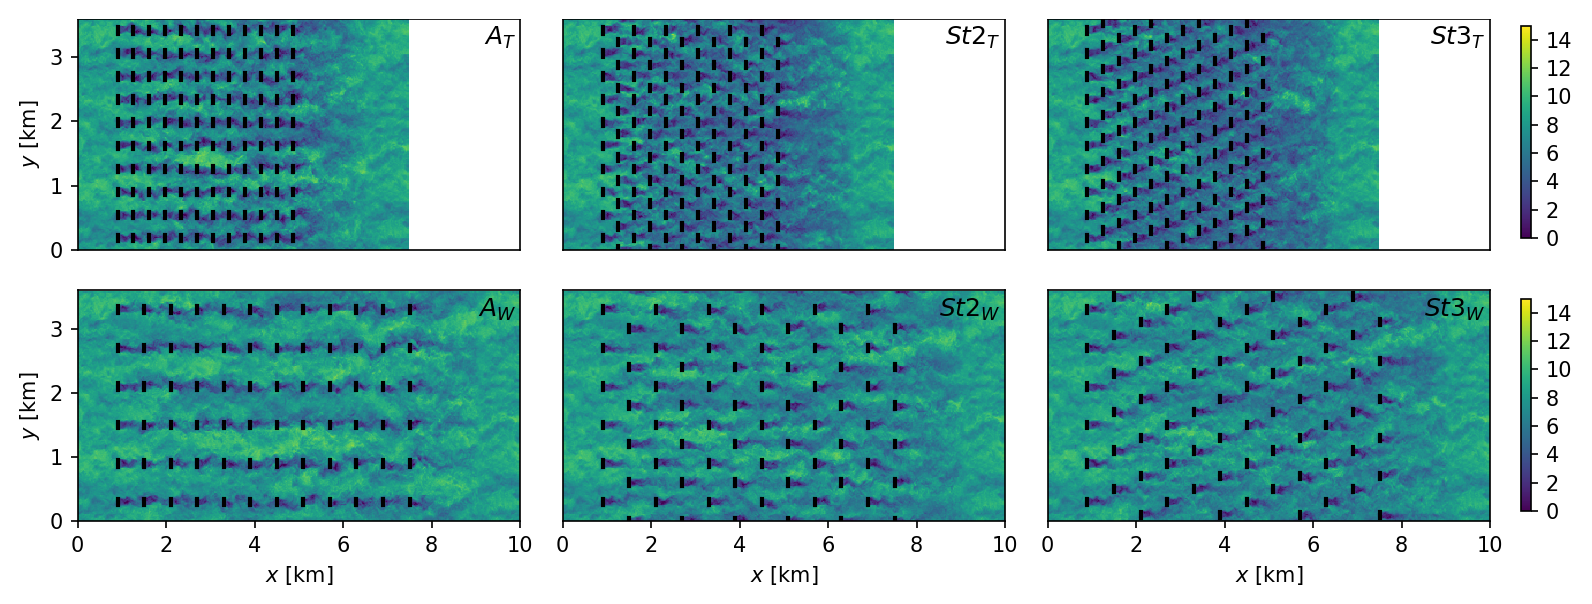
\includegraphics[width=\textwidth]{Torque18/eps/drawing.eps}
	\caption{Wind-farm layouts: (A) Aligned, (St2) Staggered every two rows, (St3) Staggered every three rows. Top: (T) Tight spacing, $S= 3.6D$. Bottom: (W) Wide spacing, $S = 6D$. Colors represent instantaneous streamwise velocity in m s$^{-1}$.\label{fig:wf_layouts}}
\end{figure}

Preliminary results of the wind-farm efficiency are shown in Figure \ref{fig:wf_effic} for reference case R and the optimal induction control case I. As expected, staggering the turbines results in higher wind-farm efficiencies for the reference cases (i.e. $St3 > St2 > A$, both for wide and tight spacing). Furthermore, by applying optimal induction control, efficiency can be increased significantly for each of the cases. Note especially case I for tight aligned layout $A_T$, which reaches the same efficiency of approximately 57\%  as the reference case R for wide aligned layout $A_W$. This observation shows that by applying dynamic induction control, the turbine density of a wind farm can be increased significantly without harming wind-farm efficiency. 
\begin{figure}
	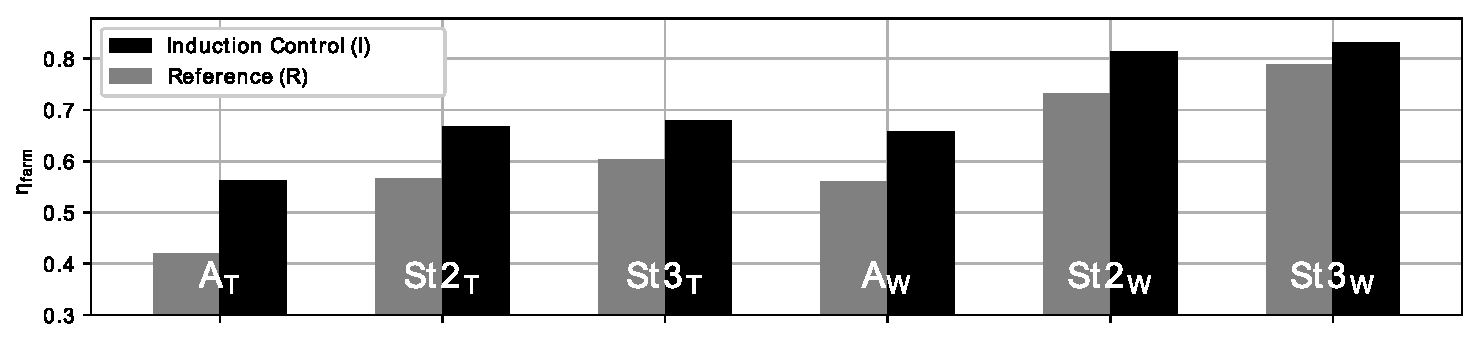
\includegraphics[width=\textwidth]{Torque18/eps/effic.eps}
	\caption{Wind-farm efficiency $\eta_{\rm farm}$ with respect to a reference case in which every turbine produces the average power of the first-row turbines in the $A_T$ layout. \label
		{fig:wf_effic}}
\end{figure}

\section{Conclusion}
The current work investigates optimal dynamic control of wind farms for a set of different wind-farm layouts and spacing. Preliminary results indicate that, through induction control, turbine density can be increased significantly without harming wind-farm efficiency. The full paper will also include the results of the yawing cases Y and IY. 


\section*{Acknowledgements}
The authors acknowledge funding by the European Research Council (ActiveWindFarms, grant no. 306471). The computational resources and services used in this work were provided by the VSC (Flemish Supercomputer Center), funded by the Research Foundation Flanders (FWO) and the Flemish Government department EWI. 

%\section*{References}
%\bibliography{\begin{thebibliography}{9}
%		\bibitem{nilsson2014large} Nilsson K, Ivanell S, Hansen K S, Mikkelsen R, S\o rensen J N, Breton S-P, Henningson D 2014 Large-eddy simulations of the Lillgrund wind farm {\it Wind Energy} {\bf 18}, pp. 449 -- 467
%		
%		\bibitem{annoni2015analysis} Annoni J, Gebraad P, Scholbrock A K, Fleming P A, van Wingerden J-W 2015 Analysis of axial-induction-based wind plant control using an engineering and a high-order wind plant model {\it Wind Energy} {\bf In press}	
%		
%		\bibitem{goit2015optimal} Goit J P and Meyers J 2015 Optimal control of energy extraction in wind-farm boundary layers {\it J Fluid Mech} {\bf 768} pp. 5--50
%		
%		\bibitem{goit2016optimal} Goit J P, Munters W and Meyers J 2016 Optimal Coordinated Control of Power Extraction in LES of a Wind Farm with Entrance Effects {\it Energies} {\bf 9}, 29
%		
%		
%%	\bibitem{goit} J. P. Goit, J. Meyers 2015, Optimal control of energy extraction in wind-farm boundary layers, J Fluid Mech 768, 5--50
%%%	\bibitem{munters} W. Munters, J. Meyers 2017, 'An optimal control framework for dynamic induction control of wind farms and their interaction with the atmospheric boundary layer', Phil Trans R Soc A 375, 20160100
%%%	\bibitem{phd} W. Munters, 'Large eddy simulations and optimal coordinated control of wind-farm boundary layers', PhD Thesis, KU Leuven, December 2017
%\end{thebibliography}


\section*{References}
\begin{thebibliography}{9}
	\bibitem{goit} J. P. Goit, J. Meyers 2015, Optimal control of energy extraction in wind-farm boundary layers, J Fluid Mech 768, 5--50
	\bibitem{munters} W. Munters, J. Meyers 2017, 'An optimal control framework for dynamic induction control of wind farms and their interaction with the atmospheric boundary layer', Phil Trans R Soc A 375, 20160100
	\bibitem{phd} W. Munters, 'Large-eddy simulations and optimal coordinated control of wind-farm boundary layers', PhD Thesis, KU Leuven, December 2017
\end{thebibliography}

\end{document}


